\documentclass[conference]{IEEEtran}
\usepackage[T1]{fontenc}
\usepackage{graphicx}
\usepackage{url}
\usepackage{algpseudocode}
\usepackage{tikz}
\usetikzlibrary{arrows.meta}
\title{SheetShrink: Efficient Spreadsheet Cleanup}
\author{
\IEEEauthorblockN{Alexander Aue-Johr}
\IEEEauthorblockA{
\textit{Institute of Rural Studies} \\
\textit{Thünen-Institute} \\
Braunschweig, Germany \\
ORCID 0009-0001-8683-3630}
}
\begin{document}
\maketitle
\begin{abstract}
Spreadsheet packages can contain large populations of empty or redundant cell records that increase storage and ingestion costs. Cleanup must distinguish this structural redundancy from small formatting or dependency witnesses that preserve required workbook behavior. We present SheetShrink, a byte-oriented OOXML cleanup system that rewrites stored XLSX packages before opening them in Excel. It combines workbook-context analysis, local rewrite decisions, compact formatting representatives, and bounded parallel execution. We define its preservation contract and separate intentional policy choices from defects. This working manuscript reports bounded implementation checks and an ongoing native-rendering validation workflow. Controlled end-to-end performance results and final corpus coverage remain to be established.
\end{abstract}
\begin{figure}[!ht]
\centering
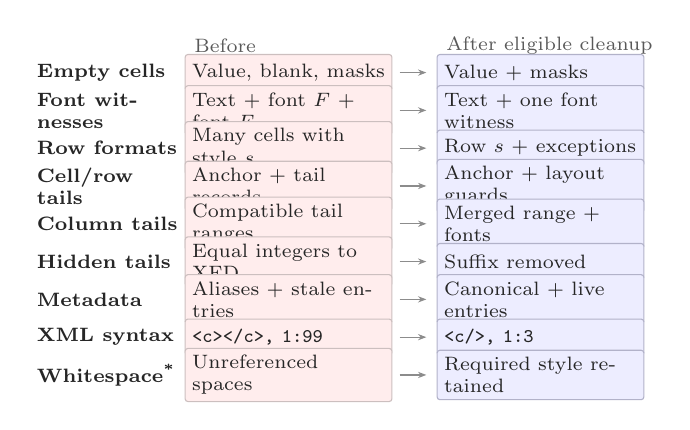
\begin{tikzpicture}[x=1cm,y=.8cm,
  source/.style={anchor=west, rounded corners=1pt,
    draw=red!20!black!25, fill=red!7, text=black!85,
    text width=2.45cm, minimum height=.46cm, inner sep=2.5pt,
    font=\scriptsize, align=left},
  result/.style={source, draw=blue!30!black!30, fill=blue!7},
  mechanism/.style={anchor=west, text width=1.8cm,
    font=\scriptsize\bfseries, align=left, text=black!85}]
\node[anchor=west,font=\scriptsize,text=black!65] at (2.0,.43) {Before};
\node[anchor=west,font=\scriptsize,text=black!65] at (5.2,.43) {After eligible cleanup};

% Each row illustrates an independent guarded transformation.
\newcommand{\cleanupcase}[4]{%
  \node[mechanism] at (0,#1) {#2};
  \node[source] at (2.0,#1) {#3};
  \draw[-{Stealth[length=3pt]},draw=black!45]
    (4.73,#1) -- (5.07,#1);
  \node[result] at (5.2,#1) {#4};
}
\cleanupcase{0}{Empty cells}
  {Value, blank, masks}
  {Value + masks}
\cleanupcase{-.60}{Font witnesses}
  {Text + font $F$ + font $F$}
  {Text + one font witness}
\cleanupcase{-1.20}{Row formats}
  {Many cells with style $s$}
  {Row $s$ + exceptions}
\cleanupcase{-1.80}{Cell/row tails}
  {Anchor + tail records}
  {Anchor + layout guards}
\cleanupcase{-2.40}{Column tails}
  {Compatible tail ranges}
  {Merged range + fonts}
\cleanupcase{-3.00}{Hidden tails}
  {Equal integers to XFD}
  {Suffix removed}
\cleanupcase{-3.60}{Metadata}
  {Aliases + stale entries}
  {Canonical + live entries}
\cleanupcase{-4.20}{XML syntax}
  {\texttt{<c></c>, 1:99}}
  {\texttt{<c/>, 1:3}}
\cleanupcase{-4.80}{Whitespace\textsuperscript{*}}
  {Unreferenced spaces}
  {Required style retained}
\end{tikzpicture}
\caption{Schematic cleanup families. Redundant cell formatting includes inherited
fills and borders. Every pair has layout, protection and dependency guards.
Row promotion requires compatible fixed-height context. Hidden-value removal
admits guarded constant tails of at least 4,096 cells ending at XFD.
\textsuperscript{*}Whitespace removal is optional. Required witnesses and
cell coordinates are retained.}
\label{fig:cleanup-overview}
\end{figure}
\section{Introduction}
An XLSX workbook can contain a small table alongside many empty cell records
and redundant row and column records. Decompressing and parsing these records
adds work. Removing every empty-looking record is
unsafe. An empty cell can preserve a border, override an inherited fill, or
influence automatic row height through its font. A whitespace value can prevent
text from extending into its neighbour. Cleanup must account for how stored records affect the workbook.

The Destatis migration workbook \texttt{wanderungen-2010120217005.xlsx}
illustrates the problem. In \texttt{Tabelle 3.4}, 21 rows contain zeros from
column L to Excel's last column, XFD, totaling 343,833 values. Removing this
hidden content requires explicit removal rules and dependency checks.
Section~\ref{sec:wanderungen} explains the rule and which values it retains.

We designed SheetShrink for use without Windows or Excel, including Python
and R workflows. Direct package processing also avoids Excel's opening cost,
which was high in our experiments.

Cleanup decisions use stored values, styles and references. SheetShrink retains
compact records needed to preserve required workbook behavior. Excel rendering
and calculated row heights are used later to validate the output.

Specialized spreadsheet parsing has demonstrated the importance of decompression,
parsing, memory use and parallel execution for data loading~\cite{sheetreader}.
Our problem adds a transformation obligation. The output remains an editable XLSX
workbook and must retain required data, dependencies and visible presentation
under a stated contract. File size alone is an inadequate measure of success.

Figure~\ref{fig:cleanup-overview} summarizes guarded reductions across cells,
rows, columns and workbook metadata. SheetShrink reuses existing style indices
and compact witnesses to preserve required effects. Native saving can additionally
compact style and shared-string tables.

The performance objective includes the complete user operation. For a sufficiently
bloated workbook, we seek to make cleanup followed by opening the cleaned file
faster than directly opening its original. A single-thread comparison
separates improvements in work performed from gains due to extra processing
resources. Parallel corpus experiments then examine throughput and memory.

\section{Preservation and Comparison Contract}
% Working prose derived from the versioned preservation contract; evaluation is pending.
\subsection{Observable spreadsheet behavior}
Cell records can contain formatting, protection, references and values that
affect other cells. SheetShrink removes redundant records while retaining those
required by its preservation contract. This paper evaluates the production
cleanup policy.

The relevant visual area includes cells with meaningful values or formulas,
visible fills or borders, and graphical objects. Row and column formats,
conditional formatting and overflowing text can also affect it. Validation covers
the union of the original and transformed areas to include removed content.
The contract permits layout changes in empty trailing rows or columns. Changes
that move or alter relevant content remain subject to validation.

\subsection{Information available before native loading}
Cleanup uses stored values, formulas, styles, references and layout attributes.
Native row heights and before/after images are available only in the separate
validation workflow. Explicit custom heights can be retained directly. For
automatic heights, an empty cell's font can require a retained representative.

An Excel-hosted alternative could measure a row, remove candidates and write the
measured height as an explicit custom height. SpreadsheetML provides a
\emph{customHeight} attribute for that policy~\cite{customheight}.

\subsection{Removal decisions and compact preservation}
SheetShrink retains a representative record when it preserves a required effect.
Examples include row-font sentinels and reuse of an existing cell style as a row
format. The checks account for inherited formatting, gaps, merges, protection
and available styles. Unresolved cases retain the required original records.

The production policy removes hidden constant tails only after dependency and
layout checks~\cite{sheetshrinkcontract}. Ordinary nonempty hidden tables remain intact, including
unreferenced values. A missing reference alone is insufficient grounds for
deleting hidden data.

\subsection{Validation and attribution boundaries}
DeltaSieve compares selected regions of independently rebuilt original and
SheetShrink workbooks in the same installed Excel
environment~\cite{deltasievecompanion}. Ordinary-save and rebuild
controls retain information for attributing differences introduced by Excel.

For XLS sources, conversion precedes the XLSX cleanup subject and has its own
failure accounting. A file requiring repair or inaccessible protected content
receives an explicit unsuccessful outcome.

Matching images establish equality within the captured regions. We evaluated
region selection using independent native reference captures and deliberately
modified test workbooks~\cite{layoutcontrols,indirectcontrols}. We retain pixel
differences and investigate their causes through repeated rendering, volatile
dependencies and capture geometry.

\section{Method}
\subsection{Representation and analysis stages}
SheetShrink removes redundant records from an XLSX ZIP package while preserving
workbook structure and cell coordinates. Before evaluating individual cells, it
reads styles, shared strings, relationships, merged regions and dependency sources.
A style index or empty value alone cannot establish redundancy.

Worksheet analysis reads decompressed bytes without creating an XML object for
each cell. A state machine distinguishes headers, columns, sheet data, merges and
the remaining XML. Tag and attribute readers track nesting and quotation marks,
preventing coordinate-like text in attribute values from being interpreted as cell
addresses. Partial markers are retained across buffer boundaries. Metadata is
retained when later decisions need it. Names, references and other interpreted
values may require decoding.

Memory use grows with worksheet size. SheetShrink retains sheet-data bytes,
analysis context and candidate metrics for later passes. Decompression, rewriting
and compression also contribute to peak memory. The supported format is
unprefixed Transitional SpreadsheetML. Unsupported namespaces, encodings and
ambiguous structures trigger preservation or exclusion~\cite{sheetshrinkcontract}.
Bounded package-header checks and declarations encountered during streaming
identify unsupported representations before opening in Excel.

Figure~\ref{fig:worksheet-states} shows how the worksheet parser dispatches column,
cell and merge readers. It retains partial state across buffer boundaries and
processes complete rows while retaining an unfinished row. Reconstruction requires
the worksheet end.
\begin{figure}[t]
\centering
\begin{tikzpicture}[x=1cm,y=1cm]
\node[state node] (seek) at (1,0) {Find root\\\texttt{worksheet}};
\node[state node] (scan) at (3.85,0) {Scan children};
\node[state final] (end) at (6.8,0) {End found};
\node[state node] (cols) at (1,-2.1) {Read columns\\\texttt{cols}};
\node[state work] (data) at (3.85,-2.1) {Read cells\\\texttt{sheetData}};
\node[state node] (merges) at (6.8,-2.1) {Read merges\\\texttt{mergeCells}};
\fill[stateSlate] (-.25,0) circle (1.5pt);
\draw[state edge] (-.25,0) -- (seek.west);
\draw[state edge] (seek) -- node[state label,above=8pt] {root found} (scan);
\draw[state edge] (scan) -- node[state label,above=8pt] {\texttt{</worksheet>}} (end);

\draw[state edge] (scan.south west) to[bend right=12]
  node[state label,above left,pos=.56] {open} (cols.north east);
\draw[state edge] (cols.north east) to[bend right=12]
  node[state label,below right,pos=.45] {close} (scan.south west);
\draw[state edge] (scan.south) to[out=-115,in=115]
  node[state label,left,pos=.5] {open} (data.north);
\draw[state edge] (data.north) to[out=65,in=-65]
  node[state label,right,pos=.5] {close} (scan.south);
\draw[state edge] (scan.south east) to[bend left=12]
  node[state label,above right,pos=.56] {open} (merges.north west);
\draw[state edge] (merges.north west) to[bend left=12]
  node[state label,below left,pos=.45] {close} (scan.south east);
\draw[state edge] (data.south west) to[out=-145,in=-35,looseness=2.3]
  node[state label,below] {emit complete rows} (data.south east);

\node[state note,text width=7.5cm,anchor=north west] at (0,-3.65)
  {Read boundaries retain state and unfinished input.};
\node[state error,text width=7.1cm,anchor=north west,minimum height=.6cm]
  at (.05,-4.15) {\textbf{Error return from unfinished states}\\
    Incomplete root/end, I/O failure or unsupported XML};
\end{tikzpicture}
\caption{The six worksheet-stream states. Child readers return to the same
worksheet dispatcher. Row-aligned progress retains a partial row across reads.
The lower box summarizes error outcomes. Reaching the end state permits
reconstruction, with workbook publication subject to its own completion checks.}
\label{fig:worksheet-states}
\end{figure}


\subsection{Parser correctness and regression controls}
The byte scanner must recognize XML structure and track parser state. It must
check element boundaries, quoted attributes, empty elements and incomplete input.
Established SAX and DOM parsers provide extensively tested syntax handling.
Memory-safe code can still misclassify content and produce an incorrect workbook.

Our development history supplies a concrete example. A Data.gov workbook used
\texttt{<v xml:space="preserve">} for visible string values. A scanner recognizing
only the literal \texttt{<v>} classified these cells as empty and removed a heading
and other strings. The correction recognizes valid element-name delimiters and
retains attributed value and inline-string elements. Negative controls reject
longer lookalike names such as \texttt{<value>}~\cite{attributedvaluefix}.
A separate defined-name regression ensures that a self-closing element cannot
consume the following paired element during replacement~\cite{definednamefix}.

The worksheet stream must reach its
closing state before output publication. An incomplete parse raises an error,
removes partial output and preserves any existing destination. Integration
fixtures exercise this failure after another worksheet has already been
processed~\cite{incompleteparsefix}. Streaming diagnostics additionally test
comments, CDATA, quotes, nesting limits and source offsets across every input
chunk size of their small fixtures.

At the time of writing, 31 correctness tests in the dedicated XML, namespace,
shared-string, range, defined-name and streaming-reader modules exercise parsing
and recognition behavior. A further 155 correctness tests in the cell, row and
tail suites cover preservation witnesses, inheritance masks and content
boundaries. Additional tests cover dependencies, styles, output construction and
execution behavior. Counts refer to test functions, with parameterized fixture
iterations counted once. The artifact records the source revision, test paths
and counting criteria.

\subsection{Effects and compact preservation witnesses}
A numeric value, formula or inline string is content. In particular, zero and a
shared-formula follower with no independent formula text remain content.
An empty cell is classified by its effective formatting in the cell, row and
column context. An explicit no-fill or borderless style can suppress a visible
inherited effect. It remains necessary whenever deletion would expose that
effect. Conversely, an explicit no-fill with nothing to clear can be redundant.
Style components and application flags are therefore interpreted together.

An empty cell's font can set automatic row height and shift later content.
SheetShrink keeps a required representative for repeated font records. Equivalent
fonts can share an identity despite different style indices. Column-font masks
and merged spans also constrain removal. A record elsewhere in the row may not
preserve a required local mask.
Figure~\ref{fig:font-witness-native} isolates the mechanism in a constructed
native Excel control. One witness preserves the observed height. Removing both
moves the next visible row.
\begin{figure}[t]
\centering
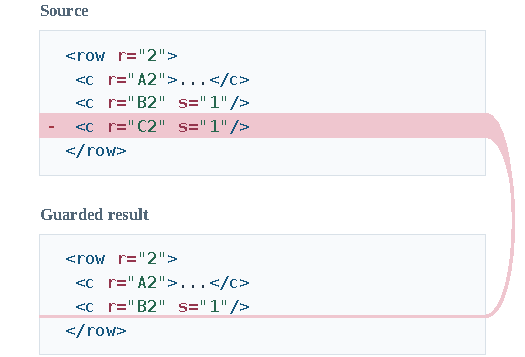
\includegraphics[width=\columnwidth]{figures/xml-methods/font-witness-code.pdf}
\par\smallskip
\begin{tabular}{@{}l@{\hspace{0.02\columnwidth}}c@{}}
Original & 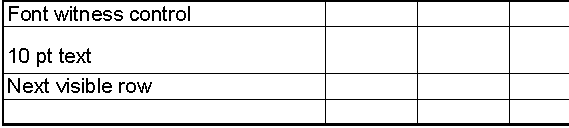
\includegraphics[width=0.70\columnwidth]{evidence/xml-methods/native-vector/font/source.pdf} \\
One witness & 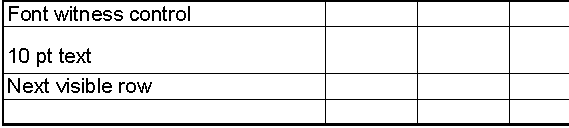
\includegraphics[width=0.70\columnwidth]{evidence/xml-methods/native-vector/font/one-witness.pdf} \\
No witness & 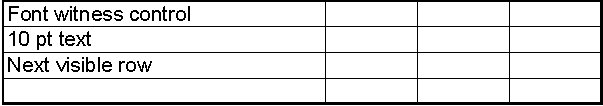
\includegraphics[width=0.70\columnwidth]{evidence/xml-methods/native-vector/font/no-witness.pdf}
\end{tabular}
\caption{Font-witness control. A2 uses Arial 10; empty B2 and C2 use Arial 18.
Retaining either blank preserves the rebuilt rendering. Removing both reduces
row 2 from 23.25 to 12.75 points and shifts the following row. XML is abbreviated;
images are native Excel print exports.}
\label{fig:font-witness-native}
\end{figure}


A fixed height eliminates this automatic-height effect, but an empty font-bearing
cell can still affect the text baseline in a row containing text. The cleaner
therefore distinguishes an empty fixed-height row from a fixed-height text row.
Protection metadata does not erase a required font contribution. Protection
formats inside the retained data extent also preserve interaction semantics,
while separately guarded exterior tails can be removed.

Other witnesses preserve relationships between coordinates. Center-across-selection
requires the contiguous blank span following the text cell. A borderless row can
mask column borders, and an empty height-bearing row can determine their vertical
extent. Column widths remain necessary when they support visible row borders.
A chart can inherit a number format from an empty first series cell. These
structures extend the preservation problem beyond the last nonempty value.
Figure~\ref{fig:fill-override-native} shows an Enron counterexample in which
Check Performance's smaller output exposes a different inherited fill. The
observation concerns the pictured rebuilt region.
\begin{figure*}[t]
\centering
\begin{tabular}{@{}c@{\hspace{0.015\textwidth}}c@{\hspace{0.015\textwidth}}c@{}}
Original & SheetShrink Default & Check Performance \\

\includegraphics[width=0.323\textwidth]{figures/xml-methods/fill-original-code.pdf} &

\includegraphics[width=0.323\textwidth]{figures/xml-methods/fill-sheetshrink-code.pdf} &

\includegraphics[width=0.323\textwidth]{figures/xml-methods/fill-check-performance-code.pdf} \\[2pt]
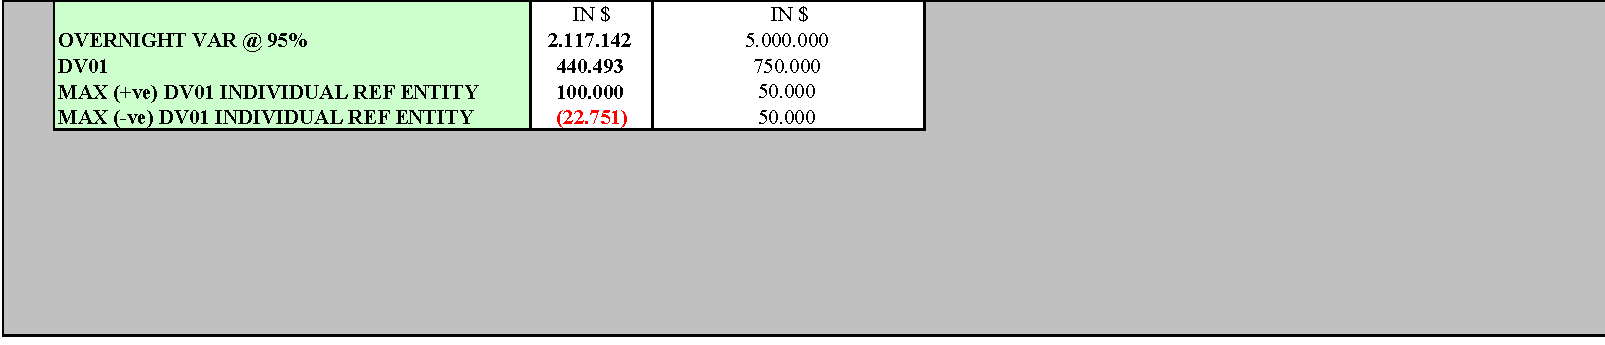
\includegraphics[width=0.323\textwidth]{evidence/xml-methods/native-vector/enron/Original.pdf} &
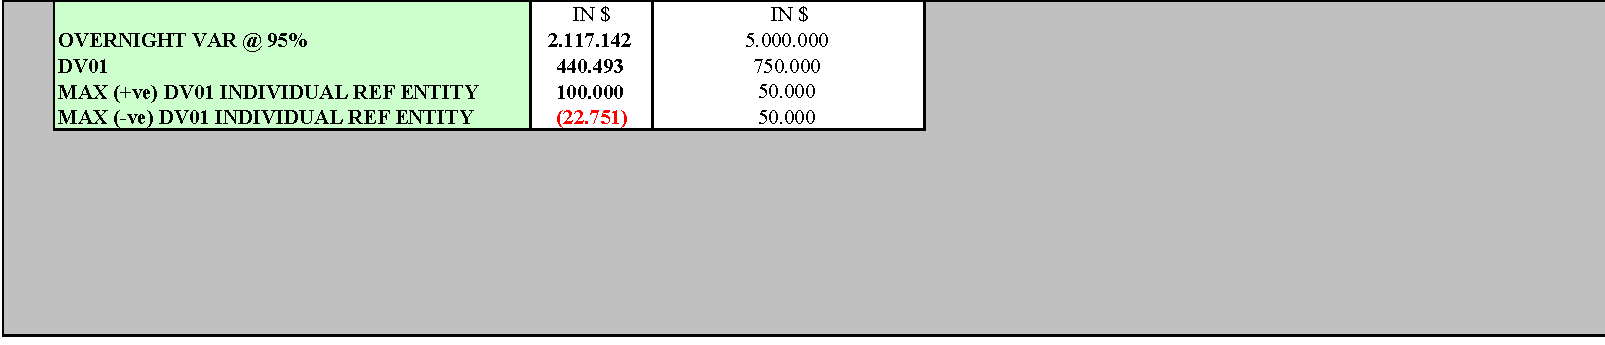
\includegraphics[width=0.323\textwidth]{evidence/xml-methods/native-vector/enron/Default.pdf} &
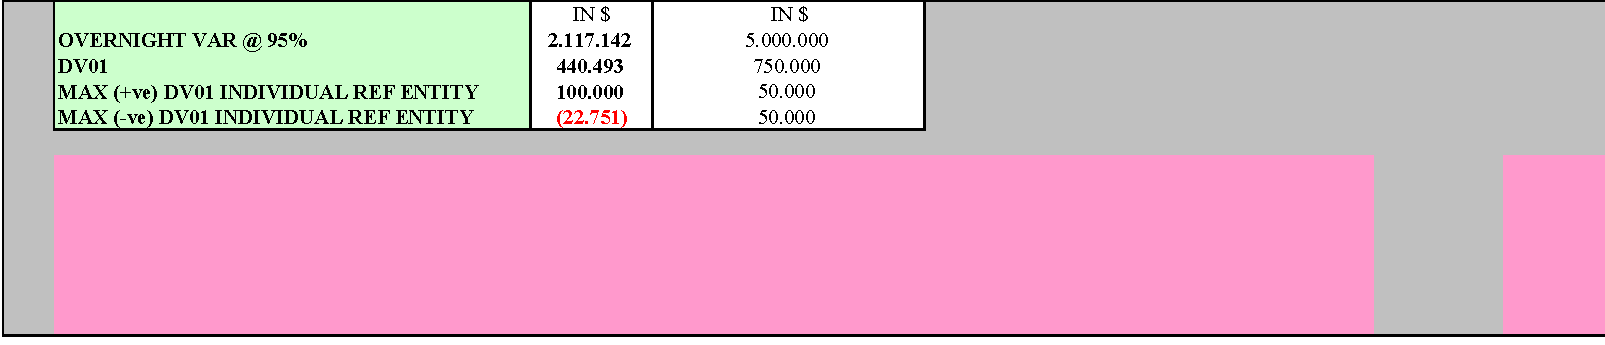
\includegraphics[width=0.323\textwidth]{evidence/xml-methods/native-vector/enron/Check-Performance.pdf}
\end{tabular}
\caption{An empty cell masks inherited formatting. In the Enron example, gray B31
overrides a pink column fill. SheetShrink preserves the mask; Check Performance
removes it and exposes pink. Native print exports match for Original and
SheetShrink after full rebuild within the displayed region. XML is abbreviated.}
\label{fig:fill-override-native}
\end{figure*}


\subsection{Guarded promotion and tail pruning}
SheetShrink can replace repeated cell styles with an existing cell style applied
to the row. The row must be visible, unprotected and have no row style. A stored
height and enabled \texttt{customHeight} flag are required. The \texttt{ht}
attribute alone permits automatic sizing. Content, merges, gaps and inherited
column formats must remain compatible with the row format.
Figure~\ref{fig:row-style-promotion} illustrates the full-width
case~\cite{rowpromotionfix}.
\begin{figure}[t]
\centering
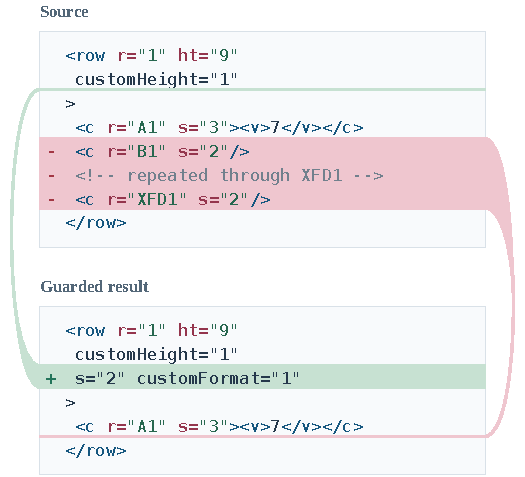
\includegraphics[width=\columnwidth]{figures/xml-methods/08-row-promotion.pdf}
\caption{Guarded dense-row promotion reuses an existing XF and keeps the value
cell. Red marks removed lines and green marks added lines. The illustration
omits the repeated middle cells. The full-width regression removes 16,383
empty cell records under the fixed-height and inheritance guards.}
\label{fig:row-style-promotion}
\end{figure}


The dominant empty-cell style occurs at least twice. Selection counts unsuitable
styles too, then applies eligibility checks. Otherwise an eligible minority
could incorrectly replace an unsuitable majority. Ties choose the smaller
existing style index. Dense promotion requires at least 1,024 occurrences.
A bounded-gap route admits at most 64 missing columns and restores required
original formats only under its inheritance checks. Sparse promotion requires
equivalent inheritance at every absent position and excludes merged sparse rows.
Uniform-fill promotion additionally checks content-cell fills. Unknown metadata
or style identities prevent promotion and retain the ordinary cleanup path.

Pruning removes formatting-only records beyond the last required content or
layout anchor. Font-only blanks beyond this boundary have no later content to
shift. Fills, borders, conditional formatting and drawings can extend the boundary.
A white row fill is redundant only if compatible column fills cover every column
through XFD. Compatible column ranges can be merged while preserving local
overrides and geometry needed for borders.

\subsection{Hidden content and the Wanderungen case}
\label{sec:wanderungen}
SheetShrink uses a conservative heuristic to remove certain hidden numeric tails.
A candidate must contain at least 4,096 identical integers and extend to XFD.
This restriction targets large repeated tails such as those in Wanderungen.
Candidates must also pass cell-level layout and dependency checks.
Gaps, formulas, text, differing values and unsupported numeric forms reject the
band. Source cells contribute before style cleanup. The common zero path compares
value bytes directly, while one admitted row span replaces per-cell entries in
the later reference map. Temporary row-local candidates still exist.

The motivating migration workbook contains 21 such zero tails in
\texttt{Tabelle 3.4}: rows 11--30 and 32, from L through XFD. Each contains
16,373 zeros, totaling 343,833. Source ZIP inspection confirms these counts and
retains the source hash. The historical cleanup investigation records 376,573
removed zeros across two worksheets, alongside 243 preserved nonzero values and
a retained short 237-zero tail~\cite{hiddentailcase}. These are content removals under an
explicit structural policy. A deliberate constant full-width matrix can meet
the same heuristic, so repetition alone does not establish user intent.

\subsection{Workbook dependencies and deferred rewriting}
SheetShrink postpones reference-sensitive deletions until it has checked supported
formulas, names, charts, objects and pivot dependencies across the workbook.
This includes references from later worksheets. Workbook relationships and sheet
scope identify reference targets. Shared-formula followers shift relative axes
and preserve absolute axes. The implementation protects enclosing referenced
ranges without enumerating each shared-formula follower's references. Dynamic
or unresolved references and unsupported expressions block deletion~\cite{sheetshrinkcurrentcontract}.

A known reference intersecting an admitted hidden span protects the entire span.
Only admitted candidates reach rewriting. Removing a payload need not remove its
format if that format still masks an inherited effect. After deferred changes,
affected rows lose their stale tail anchors and pass through cleanup again.
Otherwise records retained solely because of the removed anchor would survive
incorrectly. Whitespace removal is disabled in Default because whitespace can
control text overflow and row layout.

Package metadata has separate predicates. Calculation-chain cleanup resolves
removed cells by sheet identity and preserves unresolved mappings. The cleaner
does not evaluate formulas or manufacture replacement caches. Built-in alias
cleanup currently matches name and local scope without proving equality of the
two formula bodies.

\subsection{Parallel work and output ownership}
Figures~\ref{fig:hierarchical-scheduling} and~\ref{fig:schedule-execution}
show the task hierarchy and a schematic execution across threads. Worksheet identity remains shared across
its chunks, while ordered assembly separates execution order from output order.
\begin{figure}[t]
\centering
\begin{tikzpicture}[x=1cm,y=1cm,
  task/.style={rounded corners=2pt,draw=stateSlate!45,fill=white,
    minimum height=.48cm,inner sep=3pt,font=\scriptsize,align=center},
  edge/.style={-{Stealth[length=3pt]},draw=stateSlate!75,line width=.6pt},
  small/.style={font=\scriptsize,text=stateSlate,align=center}]
\definecolor{scheduleAmber}{HTML}{AD762B}
\path[use as bounding box] (-.45,.05) rectangle (5.55,-4.9);

\node[task,text width=1.45cm] (w1) at (1,-.45) {Workbook 1};
\node[task,text width=1.45cm] (w2) at (4,-.45) {Workbook 2};
\node[task,draw=stateBlue,fill=stateBlue!9] (a) at (.45,-1.55) {Sheet A};
\node[task,draw=stateTeal,fill=stateTeal!10] (b) at (2.1,-1.55) {Sheet B};
\node[task,draw=scheduleAmber,fill=scheduleAmber!10] (c) at (4.55,-1.55) {Sheet C};
\draw[edge] (w1) -- (a);
\draw[edge] (w1) -- (b);
\draw[edge] (w2) -- (c);
\foreach \id/\xx in {1/.7,2/2.1,3/3.5} {
  \node[task,draw=stateTeal,fill=stateTeal!10,minimum width=1cm]
    (chunk\id) at (\xx,-2.7) {B\,\id};
  \draw[edge] (b) -- (chunk\id);
}
\node[task,text width=2.45cm] (join) at (2.1,-3.8) {Assemble B\,1, B\,2, B\,3};
\foreach \id in {1,2,3} {\draw[edge] (chunk\id) -- (join);}
\node[small,anchor=north,text width=5.2cm] at (2.3,-4.25)
  {Complete rows stay together.\\Chunk results retain source order.};

\end{tikzpicture}
\caption{Task hierarchy. Workbook admission bounds active inputs; sheets and
row-aligned chunks share the Rayon pool. B\,1--B\,3 belong to one worksheet
and are assembled in source order. Colors match Figure~\ref{fig:schedule-execution}.}
\label{fig:hierarchical-scheduling}
\end{figure}

\begin{figure}[t]
\centering
\begin{tikzpicture}[x=1cm,y=1cm,
  small/.style={font=\scriptsize,text=stateSlate,align=center},
  edge/.style={-{Stealth[length=3pt]},draw=stateSlate!75,line width=.6pt}]
\definecolor{scheduleAmber}{HTML}{AD762B}
\path[use as bounding box] (0,.1) rectangle (8.3,-3.35);
\foreach \yy/\name in {-.45/1,-1.25/2,-2.05/3} {
  \draw[stateSlate!14,line width=.4pt] (1.2,\yy-.3) -- (8.1,\yy-.3);
  \node[small,anchor=east] at (1.1,\yy) {Thread \name};
}
\foreach \xx in {1.3,2.6,3.9,5.2,6.5,7.8} {
  \draw[stateSlate!10,line width=.35pt] (\xx,-.05) -- (\xx,-2.45);
}
\filldraw[fill=stateTeal!12,draw=stateTeal!65,rounded corners=1.5pt]
  (1.3,-.69) rectangle (2.15,-.21);
\node[small] at (1.725,-.45) {B init};
\filldraw[fill=stateTeal!22,draw=stateTeal,rounded corners=1.5pt]
  (2.25,-.69) rectangle (5.1,-.21);
\node[small] at (3.675,-.45) {B\,1};
\filldraw[fill=stateBlue!17,draw=stateBlue,rounded corners=1.5pt]
  (1.3,-1.49) rectangle (2.6,-1.01);
\node[small] at (1.95,-1.25) {A};
\filldraw[fill=stateTeal!38,draw=stateTeal,line width=.9pt,rounded corners=1.5pt]
  (2.7,-1.49) rectangle (5.8,-1.01);
\node[small] at (4.25,-1.25) {B\,2};
\filldraw[fill=scheduleAmber!19,draw=scheduleAmber,rounded corners=1.5pt]
  (1.3,-2.29) rectangle (2.35,-1.81);
\node[small] at (1.825,-2.05) {C};
\filldraw[fill=stateTeal!22,draw=stateTeal,rounded corners=1.5pt]
  (2.45,-2.29) rectangle (4.7,-1.81);
\node[small] at (3.575,-2.05) {B\,3};
\draw[stateTeal!65,dashed,line width=.6pt] (5.8,-2.45) -- (5.8,-.05);
\filldraw[fill=stateTeal!12,draw=stateTeal!65,rounded corners=1.5pt]
  (5.9,-.69) rectangle (7.5,-.21);
\node[small] at (6.7,-.45) {B finalize};
\node[small,anchor=north] at (5.8,-2.5) {All B chunks joined};
\draw[edge] (1.3,-3.15) -- (8.1,-3.15);
\node[small,fill=white,inner sep=2pt] at (4.7,-3.15) {Relative time};
\end{tikzpicture}
\caption{One possible execution of Figure~\ref{fig:hierarchical-scheduling}.
Chunks from one sheet can run on different threads before ordered assembly.
Bar lengths are schematic; individual steal events are not recorded.}
\label{fig:schedule-execution}
\end{figure}

Workbook, worksheet and row-chunk work share the cleanup execution budget.
A permit limits active workbooks and remains held through output finalization.
Workers can process other workbooks while one long worksheet remains active.
Large worksheets expose row-aligned chunks to Rayon, allowing idle workers to
help without splitting a row's font, promotion or tail decisions.
The chunk planner estimates byte-sized work, then adjusts boundaries to complete
rows. Small ranges use the serial path. Each chunk receives isolated metrics,
and results are assembled in source order.

Ready chunks participate in admission decisions for new worksheets. A smaller
sheet can yield admission while larger chunk work is pending. Batches retain only a bounded number of chunk results while the
assembled output grows. Workbook contexts, the output buffer and deferred
candidates remain additional memory consumers. Thread count, active-workbook
count and writer count are separate experimental parameters.

Workers compress changed worksheet members in parallel. One writer updates each
workbook's ZIP archive and publishes the completed temporary file after successful
processing. Unchanged members can reuse their compressed bytes. If every member
is unchanged, SheetShrink copies the original file byte for byte. A fast identity
check uses CRC32 and uncompressed size.

The method retains existing style and shared-string indices rather than globally
renumbering their tables. This avoids unrelated rewrites and permits copy-through
of unaffected members. It also leaves reductions requiring native save or global
table compaction outside the cleanup subject.

\section{Evaluation}
We evaluate three questions. RQ1 measures compressed-file reduction and the records
retained for preservation. RQ2 measures cleanup time, memory and total
cleanup-plus-opening time. RQ3 tests structural preservation and Excel-rendered
appearance within the stated validation scope.

\subsection{Corpus identity and outcome accounting}
Data.gov, Destatis and Enron are evaluated separately. Archive checksums, member
names and duplicate occurrences identify each corpus version. XLS conversion is
reported separately from XLSX cleanup. Recursive extraction of Internet Archive's
EDRM Enron v2 XML archives inspected nested archives and embedded containers. It
yielded 34,065 distinct SHA-256-addressed candidates, including legacy Excel files
and other OLE objects. The prepared Enron XLSX evaluation population is described
below.

For native visual stress tests, we select the 49 workbooks with the largest
absolute compressed-file reduction from each corpus, totaling 147 original
identities. Every processor baseline uses these identities. Preparation, cleanup
and visual comparison have separate outcome counts.

The frozen XLSX inventories contain 9,117 Data.gov members totaling 25.273 GB and
1,182 Destatis members totaling 2.364 GB, measured as compressed file bytes in
decimal GB. Each member has a SHA-256 identity. Outcomes distinguish completed
comparisons, differences, failures, unsupported formats and unfinished work.
Retries are counted separately. Identical packages can bypass visual comparison.
Failed captures cannot establish equality.

\subsection{Cleanup screening outcomes}
Fresh release-build runs produced 1,182 Destatis, 8,623 Data.gov, and 30,301
prepared Enron XLSX outputs. Across those outputs, aggregate compressed
file bytes fell by 15.48\%, 5.27\%, and 18.87\%, respectively.
The smaller, equal-size, and larger output counts were
1,045/30/107 for Destatis, 4,755/3,522/346 for Data.gov, and
21,565/8,415/321 for Enron. Hash checks confirmed byte identity for all
equal-size outputs in these runs. Data.gov also had 494 unsupported-namespace
skips. With sixteen workbook slots and sixteen Rayon threads, elapsed times
were 119.7, 1,134.5, and 181.6\,s, respectively, including analysis statistics
and full replay events alongside concurrent native validation~\cite{corpusdistributions}.
All three runs reached completion with zero reported processing failures.
The host used an AMD Ryzen 7 7800X3D with eight physical cores, sixteen logical
processors, 95.1\,GiB OS-visible RAM and Windows 11 Home build 26200.
Interactive replays accompany the
\href{https://alexander-aue-johr.github.io/excel-shrink-paper/replays/corpus-distributions-20261111/destatis/}{Destatis},
\href{https://alexander-aue-johr.github.io/excel-shrink-paper/replays/corpus-distributions-20261111/datagov/}{Data.gov}
and \href{https://alexander-aue-johr.github.io/excel-shrink-paper/replays/corpus-distributions-20261111/enron/}{prepared Enron XLSX}
runs; replay clocks additionally include final reporting.
Successful processing of these inputs does not establish correctness for every
valid serialization.
These descriptive results include files that grew and use only processed
input bytes as the denominator. Enron's denominator begins after
preparation. Visual preservation is evaluated separately.
Figure~\ref{fig:corpus-distributions} shows the workbook and worksheet
distributions for these runs. Empty-cell cleanup and trailing layout rows
account for prominent worksheet XML reductions. The contribution of column
range merging is especially visible in Destatis. The worksheet panels exclude
88 prepared Enron workbooks without worksheet XML observations. Workbook payload sizes use all uncompressed ZIP member sizes.
\begin{figure*}[t]
\centering
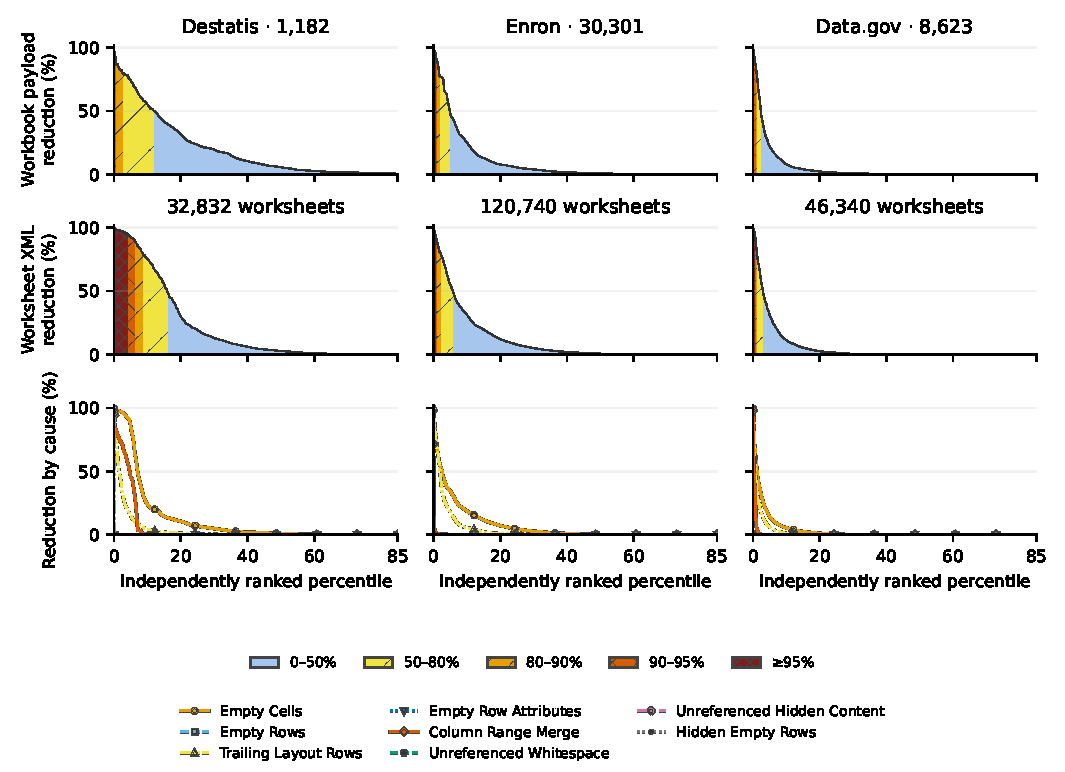
\includegraphics[width=\textwidth]{figures/corpus-uncompressed-distributions.pdf}
\caption{Full-corpus uncompressed-size reduction. Top, complete workbook
payload from all ZIP member sizes recorded in the central directory.
Middle, uncompressed worksheet XML.
Bottom, worksheet XML reduction attributed to each recorded cleanup cause.
Each curve independently sorts its observations from greatest to least
reduction. The x-axis gives the fraction of observations traversed in that
ordering. The common display ends at the 85th percentile. Remaining positive
reductions are below 0.5 percentage points. The omitted tail includes unchanged
outputs and growing workbooks (3/24/5) and worksheets (82/143/39), in
Destatis/Enron/Data.gov order, retained in the accompanying data.
Colors and hatching mark 50/80/90/95\% reduction tiers.
Data.gov's 494 unsupported-namespace
inputs are excluded from these processed-output distributions. The worksheet
panels cover 1,182 Destatis, 30,213 Enron and 8,623 Data.gov workbooks with
recorded worksheet XML. Enron begins with prepared XLSX inputs.}
\label{fig:corpus-distributions}
\end{figure*}

Among 9,117 Data.gov inputs, 493 workbooks contained explicitly prefixed
worksheet data elements. After experimental namespace normalization and Default
cleanup, only two produced smaller compressed packages, by 6.415\% and 0.047\%
relative to the normalized baseline. Cell-record removal in other outputs did
not reduce package size~\cite{prefixeddataexperiment}.

Corpus testing exposed parsing and preservation defects. Enron controls identified
missing center-across-selection spans and fill masks by restoring the affected
original cell records. These findings informed regression fixtures and native
Excel controls that complement the screening results~\cite{enrondefaultcontrols}.

\subsection{Sampling and reference controls}
We select the random sample from a frozen eligible population using a recorded
seed before inspecting visual results. Sampling strata reflect corpus, package
size and structural features known before validation. Low-reduction and unchanged
files remain included. A separately labelled development stress set contains large
and historically problematic workbooks.

Where feasible, sampled files receive full native reference captures of the
relevant visual area, independently of the candidate selector. Timeouts remain in
the denominator, without substituting easier workbooks. Test mutations introduce
known visible changes to values, styles, geometry, conditional dependencies and
objects. Changes normalized away by Excel are reported separately.

\subsection{Performance and comparison subjects}
We compared direct open--save trials with fresh six-worker SheetShrink cleanup
followed by the same library. Across the two displayed laptop workbooks, all 33 SheetShrink
trials completed under a 4\,GiB commit limit, compared with 21 original trials.
Median elapsed time improved in all seven fully completed pairs. Migration
with openpyxl took 111.3\,s directly and 9.7\,s including cleanup.

Tables~\ref{tab:case-study-transformations} and
\ref{tab:case-study-resources} join the opening/memory case study through frozen
file identities. The full experiment retains 288 opening/saving attempts
across six variants and three repetitions. The selected
Enron workbook has a separate eighteen-attempt follow-up on the larger-memory
host, described below. Its measurements retain their own host and configuration.
The tables display Migration and QT/RR, with Enron size evidence and a separate
resource follow-up.
The payload table uses exact retained comparator outputs and separately regenerated
Sheet Shrink controls with verified native-candidate member identities. Per-trial
member inventories of timed fresh outputs were not retained. Native pixel counts
are reported only for measured, retained image pairs with matched origins.
Missing scopes and image-size differences remain explicit.

The compact resource table reports total elapsed time and library working-set
peaks. The artifact separately retains pipeline working sets and job-commit
peaks. Each displayed time is a median of completed attempts,
with memory maxima over all three attempts. Stopped attempts retain their
elapsed time and memory boundary. Existing prepared-output
variants measure subsequent library processing. Fresh Sheet Shrink rows include
cleanup within the measured pipeline. The common host is a Ryzen 5 4500U laptop
with six logical processors, 8 GiB installed RAM and Windows 11. Each job has a
4 GiB commit cap and a 900 s timeout, with the free-RAM reserve disabled.
The Sheet Shrink executable is frozen at revision \texttt{765c480} and uses six
Rayon and six writer workers. Native visual observations use the retained
paired-rebuild protocol.

\begin{table*}[t]
\centering
\footnotesize
\setlength{\tabcolsep}{2.5pt}
\renewcommand{\arraystretch}{1.08}
\caption{Selected-case uncompressed payload reduction and retained native pixel evidence. Payload is the sum of all ZIP-member sizes in decimal MB. Image-pair counts state measured/recorded coverage.}
\label{tab:case-study-transformations}
\begin{tabular}{lrl}
\hline
Variant & Payload MB (reduction) & Changed / compared pixels; coverage \\
\hline
\multicolumn{3}{l}{\textbf{Destatis Migration}} \\
Original & \CasePairBars[4.4]{248.39 (0\%)}{1.09990}{1.09990}{casebarblue} & Reference \\
SheetShrink\textsuperscript{*} & \CasePairBars[4.4]{16.46 (93\%)}{1.09990}{0.07288}{casebarblue} & \begin{tabular}[c]{@{}l@{}}0 / 101,874,379\\37/38 image pairs\\5 size differences\\Normalized baseline\end{tabular} \\
NXPowerLite & \CasePairBars[4.4]{197.48 (20\%)}{1.09990}{0.87447}{casebarblue} & Failed \\
XLStylesTool & \CasePairBars[4.4]{248.42 (-0.0095\%)}{1.09990}{1.10000}{casebarorange} & Failed \\
Check Performance & \CasePairBars[4.4]{20.15 (92\%)}{1.09990}{0.08922}{casebarblue} & Memory limit \\
Inquire & \CasePairBars[4.4]{116.44 (53\%)}{1.09990}{0.51559}{casebarblue} & Failed \\
\hline
\multicolumn{3}{l}{\textbf{Data.gov QT/RR}} \\
Original & \CasePairBars[4.4]{1350.77 (0\%)}{1.10000}{1.10000}{casebarblue} & Reference \\
SheetShrink\textsuperscript{*} & \CasePairBars[4.4]{29.91 (98\%)}{1.10000}{0.02436}{casebarblue} & No capture regions \\
NXPowerLite & \CasePairBars[4.4]{29.98 (98\%)}{1.10000}{0.02442}{casebarblue} & No capture regions \\
XLStylesTool & \CasePairBars[4.4]{1350.77 (-7.8e-05\%)}{1.10000}{1.10000}{casebarorange} & No capture regions \\
Check Performance & \CasePairBars[4.4]{25.59 (98\%)}{1.10000}{0.02084}{casebarblue} & No capture regions \\
Inquire & \CasePairBars[4.4]{30.13 (98\%)}{1.10000}{0.02454}{casebarblue} & No completed report \\
\hline
\multicolumn{3}{l}{\textbf{Enron b2d0dfef}} \\
Original & \CasePairBars[4.4]{353.15 (0\%)}{1.09999}{1.09999}{casebarblue} & Reference \\
SheetShrink\textsuperscript{*} & \CasePairBars[4.4]{2.58 (99\%)}{1.09999}{0.00804}{casebarblue} & No retained pairs (0/2824) \\
NXPowerLite & \CasePairBars[4.4]{2.55 (99\%)}{1.09999}{0.00795}{casebarblue} & \begin{tabular}[c]{@{}l@{}}6,437 / 11,640,701,446\\1033/1033 image pairs\end{tabular} \\
XLStylesTool & \CasePairBars[4.4]{353.16 (-0.0011\%)}{1.09999}{1.10000}{casebarorange} & No capture regions \\
Check Performance & \CasePairBars[4.4]{2.54 (99\%)}{1.09999}{0.00792}{casebarblue} & \begin{tabular}[c]{@{}l@{}}456,503 / 46,890,576\\8/1032 image pairs\\2 size differences\end{tabular} \\
Inquire & \CasePairBars[4.4]{2.57 (99\%)}{1.09999}{0.00801}{casebarblue} & \begin{tabular}[c]{@{}l@{}}9,739 / 11,728,328,854\\1040/1040 image pairs\\1040 size differences\end{tabular} \\
\hline
\end{tabular}
\par\smallskip
\begin{minipage}{0.98\textwidth}\footnotesize \textsuperscript{*}SheetShrink uses separately regenerated controls whose uncompressed members match the native candidates; full per-trial member inventories of the timed pipelines were not retained. Wanderungen uses a normalized baseline. Counts compare exact RGBA values in common rectangles with matched origins; overlapping captures can count pixels repeatedly. Image-size differences remain separate from common-area pixel counts. Different plans and incomplete scopes preclude a cross-tool preservation ranking. No capture regions or retained pairs provide no pixel-equality observation. Gray bars show the original; blue/orange show payload at or below/above the original. Input/output hashes, scope details and failures remain in the artifact.\end{minipage}
\end{table*}

\begin{table*}[p]
\centering
\footnotesize
\setlength{\tabcolsep}{2.5pt}
\renewcommand{\arraystretch}{1.08}
\caption{Opening/saving observations on two hosts. Cells show median total seconds above maximum memory across three attempts. Host blocks specify commit caps and memory metrics. The timeout is 900 s.}
\label{tab:case-study-resources}
\begin{tabular}{lrrrrrr}
\hline
Endpoint & Original & SheetShrink & NXPowerLite & XLStylesTool & \shortstack{Check\\Performance} & Inquire \\
\multicolumn{7}{l}{\textbf{Ryzen 5 4500U laptop: 4 GiB commit cap; library working set (MiB)}} \\
\hline
\multicolumn{7}{l}{\textbf{Destatis Migration}} \\
openpyxl & \shortstack[r]{\CasePairBars[2.2]{111.30}{1.10000}{1.10000}{casebarblue}\\\CasePairBars[2.2]{2700}{1.09997}{1.09997}{casebarblue}} & \shortstack[r]{\CasePairBars[2.2]{9.67}{1.10000}{0.09555}{casebarblue}\\\CasePairBars[2.2]{250}{1.09997}{0.10194}{casebarblue}} & \shortstack[r]{\CasePairBars[2.2]{83.58}{1.10000}{0.82602}{casebarblue}\\\CasePairBars[2.2]{1996}{1.09997}{0.81334}{casebarblue}} & \shortstack[r]{\CasePairBars[2.2]{111.13}{1.10000}{1.09829}{casebarblue}\\\CasePairBars[2.2]{2700}{1.09997}{1.10000}{casebarorange}} & \shortstack[r]{\CasePairBars[2.2]{9.11}{1.10000}{0.09002}{casebarblue}\\\CasePairBars[2.2]{236}{1.09997}{0.09603}{casebarblue}} & \shortstack[r]{\CasePairBars[2.2]{54.96}{1.10000}{0.54318}{casebarblue}\\\CasePairBars[2.2]{1530}{1.09997}{0.62347}{casebarblue}} \\
pandas to XLSX & \shortstack[r]{\colorbox{caseadverse}{\strut M}\\3900} & \shortstack[r]{35.83\\856} & \shortstack[r]{\colorbox{caseadverse}{\strut M}\\3900} & \shortstack[r]{\colorbox{caseadverse}{\strut M}\\3900} & \shortstack[r]{\colorbox{caseadverse}{\strut M}\\3900} & \shortstack[r]{\colorbox{caseadverse}{\strut M}\\3900} \\
pandas to CSV & \shortstack[r]{\colorbox{caseadverse}{\strut M}\\3900} & \shortstack[r]{11.54\\214} & \shortstack[r]{\colorbox{caseadverse}{\strut M}\\3900} & \shortstack[r]{\colorbox{caseadverse}{\strut M}\\3900} & \shortstack[r]{\colorbox{caseadverse}{\strut M}\\3900} & \shortstack[r]{\colorbox{caseadverse}{\strut M}\\3900} \\
Excel COM & \shortstack[r]{\CasePairBars[2.2]{20.34}{1.10000}{1.10000}{casebarblue}\\\CasePairBars[2.2]{429}{1.10000}{1.10000}{casebarblue}} & \shortstack[r]{\CasePairBars[2.2]{9.92}{1.10000}{0.53635}{casebarblue}\\\CasePairBars[2.2]{309}{1.10000}{0.79239}{casebarblue}} & \shortstack[r]{\CasePairBars[2.2]{17.94}{1.10000}{0.96972}{casebarblue}\\\CasePairBars[2.2]{409}{1.10000}{1.04743}{casebarblue}} & \shortstack[r]{\CasePairBars[2.2]{20.17}{1.10000}{1.09070}{casebarblue}\\\CasePairBars[2.2]{428}{1.10000}{1.09743}{casebarblue}} & \shortstack[r]{\CasePairBars[2.2]{5.34}{1.10000}{0.28867}{casebarblue}\\\CasePairBars[2.2]{259}{1.10000}{0.66287}{casebarblue}} & \shortstack[r]{\CasePairBars[2.2]{9.99}{1.10000}{0.53998}{casebarblue}\\\CasePairBars[2.2]{324}{1.10000}{0.83184}{casebarblue}} \\
R openxlsx & \shortstack[r]{\CasePairBars[2.2]{44.38}{1.08690}{1.08690}{casebarblue}\\\CasePairBars[2.2]{824}{1.09028}{1.09028}{casebarblue}} & \shortstack[r]{\CasePairBars[2.2]{13.70}{1.08690}{0.33547}{casebarblue}\\\CasePairBars[2.2]{317}{1.09028}{0.41938}{casebarblue}} & \shortstack[r]{\CasePairBars[2.2]{30.04}{1.08690}{0.73571}{casebarblue}\\\CasePairBars[2.2]{684}{1.09028}{0.90437}{casebarblue}} & \shortstack[r]{\CasePairBars[2.2]{44.92}{1.08690}{1.10000}{casebarorange}\\\CasePairBars[2.2]{831}{1.09028}{1.10000}{casebarorange}} & \shortstack[r]{\CasePairBars[2.2]{11.70}{1.08690}{0.28648}{casebarblue}\\\CasePairBars[2.2]{286}{1.09028}{0.37824}{casebarblue}} & \shortstack[r]{\CasePairBars[2.2]{32.22}{1.08690}{0.78900}{casebarblue}\\\CasePairBars[2.2]{564}{1.09028}{0.74618}{casebarblue}} \\
R readxl + writexl & \shortstack[r]{\colorbox{caseadverse}{\strut M}\\4070} & \shortstack[r]{178.17\\262} & \shortstack[r]{\colorbox{caseadverse}{\strut M}\\4070} & \shortstack[r]{\colorbox{caseadverse}{\strut M}\\4070} & \shortstack[r]{\colorbox{caseadverse}{\strut M}\\4072} & \shortstack[r]{\colorbox{caseadverse}{\strut M}\\4072} \\
\hline
\multicolumn{7}{l}{\textbf{Data.gov QT/RR}} \\
openpyxl & \shortstack[r]{\colorbox{caseadverse}{\strut M}\\3913} & \shortstack[r]{19.84\\318} & \shortstack[r]{12.26\\299} & \shortstack[r]{\colorbox{caseadverse}{\strut M}\\3913} & \shortstack[r]{12.07\\299} & \shortstack[r]{12.39\\303} \\
pandas to XLSX & \shortstack[r]{\CasePairBars[2.2]{249.13}{1.10000}{1.10000}{casebarblue}\\\CasePairBars[2.2]{327}{1.04035}{1.04035}{casebarblue}} & \shortstack[r]{\CasePairBars[2.2]{22.99}{1.10000}{0.10151}{casebarblue}\\\CasePairBars[2.2]{346}{1.04035}{1.10000}{casebarorange}} & \shortstack[r]{\CasePairBars[2.2]{15.79}{1.10000}{0.06972}{casebarblue}\\\CasePairBars[2.2]{327}{1.04035}{1.03958}{casebarblue}} & \shortstack[r]{\CasePairBars[2.2]{246.68}{1.10000}{1.08915}{casebarblue}\\\CasePairBars[2.2]{327}{1.04035}{1.03929}{casebarblue}} & \shortstack[r]{\CasePairBars[2.2]{15.55}{1.10000}{0.06864}{casebarblue}\\\CasePairBars[2.2]{327}{1.04035}{1.03987}{casebarblue}} & \shortstack[r]{\CasePairBars[2.2]{16.09}{1.10000}{0.07103}{casebarblue}\\\CasePairBars[2.2]{327}{1.04035}{1.03944}{casebarblue}} \\
Excel COM & \shortstack[r]{\CasePairBars[2.2]{39.79}{0.70004}{0.70004}{casebarblue}\\\CasePairBars[2.2]{929}{1.09853}{1.09853}{casebarblue}} & \shortstack[r]{\CasePairBars[2.2]{11.84}{0.70004}{0.20838}{casebarblue}\\\CasePairBars[2.2]{272}{1.09853}{0.32148}{casebarblue}} & \shortstack[r]{\CasePairBars[2.2]{4.67}{0.70004}{0.08223}{casebarblue}\\\CasePairBars[2.2]{253}{1.09853}{0.29933}{casebarblue}} & \shortstack[r]{\CasePairBars[2.2]{39.02}{0.70004}{0.68650}{casebarblue}\\\CasePairBars[2.2]{931}{1.09853}{1.10000}{casebarorange}} & \shortstack[r]{\CasePairBars[2.2]{62.52}{0.70004}{1.10000}{casebarorange}\\\CasePairBars[2.2]{246}{1.09853}{0.29069}{casebarblue}} & \shortstack[r]{\CasePairBars[2.2]{4.77}{0.70004}{0.08385}{casebarblue}\\\CasePairBars[2.2]{247}{1.09853}{0.29152}{casebarblue}} \\
R openxlsx & \shortstack[r]{\CasePairBars[2.2]{140.86}{1.10000}{1.10000}{casebarblue}\\\CasePairBars[2.2]{2453}{1.09990}{1.09990}{casebarblue}} & \shortstack[r]{\CasePairBars[2.2]{11.28}{1.10000}{0.08812}{casebarblue}\\\CasePairBars[2.2]{242}{1.09990}{0.10870}{casebarblue}} & \shortstack[r]{\CasePairBars[2.2]{4.26}{1.10000}{0.03324}{casebarblue}\\\CasePairBars[2.2]{224}{1.09990}{0.10044}{casebarblue}} & \shortstack[r]{\CasePairBars[2.2]{140.40}{1.10000}{1.09640}{casebarblue}\\\CasePairBars[2.2]{2454}{1.09990}{1.10000}{casebarorange}} & \shortstack[r]{\CasePairBars[2.2]{3.55}{1.10000}{0.02770}{casebarblue}\\\CasePairBars[2.2]{210}{1.09990}{0.09434}{casebarblue}} & \shortstack[r]{\CasePairBars[2.2]{4.32}{1.10000}{0.03375}{casebarblue}\\\CasePairBars[2.2]{225}{1.09990}{0.10065}{casebarblue}} \\
R readxl + writexl & \shortstack[r]{\CasePairBars[2.2]{11.90}{1.10000}{1.10000}{casebarblue}\\\CasePairBars[2.2]{1341}{1.10000}{1.10000}{casebarblue}} & \shortstack[r]{\CasePairBars[2.2]{10.06}{1.10000}{0.93020}{casebarblue}\\\CasePairBars[2.2]{258}{1.10000}{0.21204}{casebarblue}} & \shortstack[r]{\CasePairBars[2.2]{2.94}{1.10000}{0.27160}{casebarblue}\\\CasePairBars[2.2]{240}{1.10000}{0.19675}{casebarblue}} & \shortstack[r]{\CasePairBars[2.2]{11.89}{1.10000}{1.09963}{casebarblue}\\\CasePairBars[2.2]{1340}{1.10000}{1.09966}{casebarblue}} & \shortstack[r]{\CasePairBars[2.2]{2.88}{1.10000}{0.26619}{casebarblue}\\\CasePairBars[2.2]{248}{1.10000}{0.20355}{casebarblue}} & \shortstack[r]{\CasePairBars[2.2]{2.96}{1.10000}{0.27394}{casebarblue}\\\CasePairBars[2.2]{239}{1.10000}{0.19643}{casebarblue}} \\
\hline
\multicolumn{7}{l}{\textbf{Ryzen 7 7800X3D: 24 GiB commit cap; process-tree commit (GiB)}} \\
\multicolumn{7}{l}{\textbf{Destatis Migration}} \\
pandas to XLSX & \shortstack[r]{\colorbox{caseadverse}{\strut M}\\24.00} & \shortstack[r]{24.729\\1.27} & -- & -- & -- & -- \\
pandas to CSV & \shortstack[r]{\colorbox{caseadverse}{\strut M}\\24.00} & \shortstack[r]{8.291\\0.65} & -- & -- & -- & -- \\
R readxl + writexl & \shortstack[r]{392.149\\8.70} & \shortstack[r]{131.953\\0.51} & -- & -- & -- & -- \\
\hline
\multicolumn{7}{l}{\textbf{Data.gov QT/RR}} \\
openpyxl & \shortstack[r]{279.638\\12.56} & \shortstack[r]{11.519\\3.66} & -- & -- & -- & -- \\
\hline
\end{tabular}
\par\smallskip
\begin{minipage}{0.98\textwidth}\footnotesize SheetShrink includes fresh cleanup through library exit. Other columns measure processing of prepared outputs, with their cleanup excluded. Completed cells have three successful attempts. M means all three attempts stopped at the memory limit, with reached memory retained below. Bars compare original (gray) and measured value (blue at or below, orange above) on a common linear scale per endpoint and metric, requiring completed originals. RSS covers library phases, with nominal 20 ms sampling. Pipeline working sets, OS job-commit peaks, cleanup/open/save phases, stopped elapsed times, CPU, ranges and all 288 receipts remain in the artifact. The larger-host block reports aggregate process-tree commit in GiB, including cleanup. Dashes indicate unmeasured conditions.\end{minipage}
\end{table*}


\subsection{Larger-memory-host follow-up}
We repeated the four workbook/library combinations that reached the laptop's
4\,GiB commit limit on an AMD Ryzen 7 7800X3D with sixteen logical processors and
95.1\,GiB of usable RAM. Each combination received three Original and three fresh
SheetShrink trials at both 4\,GiB and 24\,GiB process-tree commit limits, totaling
48 trials. The same SheetShrink binary uses sixteen Rayon and sixteen writer
workers, with one active workbook. Trials reserve 8\,GiB of physical RAM and
commit headroom and time out after 900 seconds. Software versions are Python
3.12.14, openpyxl 3.1.5, pandas 3.0.1, R 4.6.2, readxl 1.6.0 and
writexl 2.0.1~\cite{openmemoryfollowup}.

At 4\,GiB, all twelve Original trials reached the memory limit, while all twelve
fresh-cleanup pipelines completed. At 24\,GiB, all six Original trials for
Migration/readxl and QT/RR/openpyxl completed, while Migration's six pandas trials
reached the limit. All twelve fresh-cleanup pipelines completed. The artifact
retains completed and memory-limited results. Trials stopped for memory receive
no runtime ratio. For Migration/readxl and QT/RR/openpyxl, cleanup plus processing
was 2.97 and 24.28 times faster, respectively, taking 131.953 versus 392.149 s and
11.519 versus 279.638 s.

The higher memory limit lets some previously memory-limited trials complete,
allowing runtime comparisons. Native visual comparisons, another cleanup benchmark
and read-only evidence analysis ran concurrently, with filesystem caches retained.
The ratios describe paired results under these conditions. Sampled physical RAM
and commit headroom stayed above the declared reserve throughout all 48 trials.

After timing, regenerated controls for both inputs matched the native candidates'
uncompressed member names, lengths and SHA-256 hashes. Migration uses a documented
normalized baseline. QT/RR's selected capture plan contains no captures. Timed
fresh outputs retain archive hashes, without full member inventories. Each
completed fresh pipeline was followed by a second cleanup outside the timed
interval. Its ZIP identity flags do not establish general cleanup idempotence.

\subsection{Enron selected-case follow-up}
\label{sec:enron-open-save-followup}
The Enron case uses the Enron workbook whose original SHA-256 begins
\texttt{7298df9a6a76}. Its original archive contains 42,710,945 compressed
bytes and 353,151,842 uncompressed member bytes. On the same larger-memory
host, six variants each received three openpyxl 3.1.5 round-trip attempts,
with a 4\,GiB process-tree commit limit, an 8\,GiB physical-RAM and commit
reserve and a 300-second timeout~\cite{enronopenmemory}.
Original and XLStylesTool
reached the memory limit in all three attempts. Fresh SheetShrink cleanup
followed by the library round trip completed with a median process-creation-to-exit
time of 3.021 seconds and a maximum job-commit peak of 891.4\,MiB.
Prepared Check Performance, Inquire and NXPowerLite outputs completed their
library round trips with respective medians of 1.036, 1.054 and 1.101 seconds,
and maximum job-commit peaks of approximately 535.6\,MiB.

The external prepared-output endpoints omit their tools' preparation cost.
The SheetShrink endpoint includes fresh cleanup, so these observations do
not establish an end-to-end speed ranking among cleaners. Memory-limited
attempts remain censored. Recorded commit peaks slightly exceed the configured
4\,GiB boundary and are retained without clamping. Concurrent native
comparisons and retained filesystem caches qualify this selected-case result.
After the timed series, a separate fresh SheetShrink control matched all
eighteen uncompressed member names, lengths and hashes of the retained native
candidate. Its output has 384,724 compressed bytes and 2,581,673 uncompressed
member bytes. This representative identity check links the control to the
visual audit, while preserving that audit's selected-coverage limitations.
The timed trials retain archive hashes, without full per-trial member inventories.


\subsection{Distributed comparator measurements}
We distribute native tool comparisons across Windows hosts because opening,
cleanup and saving are costly. Each result records its host, input identity,
configuration and timing boundary. Cross-tool ratios compare the same original
workbook with SheetShrink on the same host. Each host/tool combination is plotted
separately. Workload, tool behavior and session conditions still affect these
ratios. The frozen selection comprises the 49 workbooks with the largest absolute
compressed-file savings in each corpus's earlier SheetShrink screening. Results
apply to these selected cases.

NXPowerLite runs on a Lenovo 81YQ with a Ryzen 5 4500U (six cores and six logical
processors), 8 GiB installed RAM (7.37 GiB usable), a 512 GB Samsung MZALQ512HALU
NVMe SSD and Windows 11 Home build 26200. The power scheme is Energy Star.
Resource records include other open Excel and validation processes.

\paragraph{Comparator configuration}
NXPowerLite Desktop 11.0.1 x64 uses a custom Excel profile with only excess
cell-formatting cleanup enabled. All other cleanup options are disabled to
preserve visible content. An output audit checks whether images remain unchanged.

We compare media, drawings, charts and embedded objects byte-for-byte against the
originals. Of 147 workbooks, 129 became smaller and ten remained unchanged. Eight
Enron inputs failed with an internal NXPowerLite error, including after restarting
and retrying. Five outputs recompressed PNGs without changing decoded RGBA pixels
or dimensions. Another changed an embedded Word document. These six outputs are
retained separately and excluded from the formatting-focused timing figure. The
remaining 133 outputs passed the audit. Worksheet appearance still requires
separate visual validation.

XLStylesTool UWP 3.0.1.0 runs on the same host, with forced style normalization,
name unhiding and wholesale external-name removal disabled. We retain 122
hash-matched inputs with confirmed primary conversions and complete timing and
resource records. The other 25 inputs lack complete timing evidence and are
excluded. All 122 outputs preserve audited media and object parts byte-for-byte.
The joint figure uses the 110 inputs shared by both tools, comprising 21 Destatis,
41 Enron and 48 Data.gov workbooks, with the same repeated SheetShrink baselines.
Table~\ref{tab:top49-resources} reports NXPowerLite resources for all 133 audited
outputs.

Check Performance uses Excel 16.0.20527.20150 on the Lenovo host, with one
owned private-desktop Excel worker per input. Among the same 110 originals,
102 primary workflows completed (86 confirmed Optimize All actions and sixteen
no-optimization-needed outcomes), one was partial and seven failed, including
one timeout. Complete outcomes comprise 21 Destatis, 36 Enron and 45 Data.gov
inputs. The partial attempt saved an output before a progress-record replacement
failed; its successful diagnostic retry remains separate from primary statistics.
All original hashes matched before and after processing.

Check Performance wall time covers native-wrapper startup through exit,
including control saves, optimization, artifact creation and shutdown. Input
staging and independent hashing are excluded. Optimization and its associated
saves share one phase; their individual times are unavailable. Excel-only CPU
was retained through exit for all complete primaries, with working set and
private bytes sampled at a median mean interval of 251 ms. All 990 reused Lenovo
SheetShrink measurements list a concurrent Check Performance runner process;
these snapshots do not establish whether it was active. The median descriptive
workflow ratios are 20.19, 22.75 and 4.84 for Destatis, Enron and Data.gov.
Background-load uncertainty and different endpoints qualify these ratios.

The Inquire lane uses an HP EliteBook 645 G11 with an AMD Ryzen 5 PRO 7535U
(six physical cores, twelve logical processors), 32 GiB installed RAM,
a 512 GB SOLIDIGM NVMe SSD and Windows 11 Enterprise build 26200.9711.
Excel and Inquire file versions are 16.0.17932.21056 and 16.0.16626.20076.
Of the same 110 originals, 90 have full primary Inquire successes, six partial
outcomes and fourteen failures. Diagnostic retries remain separate. Full
successes comprise 19 Destatis, 28 Enron and 43 Data.gov workbooks.

Inquire records single historical Excel workflow observations, including opening,
cleanup with internal saving, explicit saving and shutdown; detailed boundaries
remain in the per-case receipts. Partial and failed attempts receive no
completed-runtime ratio. Historical hardware and version attribution partly
uses execution-session provenance and later inventory rather than per-trial
capture. Among the 90 complete pairs, 41 Inquire work directories were on local
NVMe, 48 on a USB-connected Samsung 870 QVO SSD, and one has incomplete storage
attribution. All paired SheetShrink trials used local NVMe. The source receipts retain these storage conditions. The median descriptive workflow
ratios are 19.36, 15.18 and 12.04 for Destatis, Enron and Data.gov, respectively.
Different endpoints and storage conditions constrain their interpretation.

The HP SheetShrink lane freezes revision \texttt{75e85035}, twelve Rayon and
twelve writer workers, and one active workbook. One warm-up precedes seven
measured trials per input, extended to eleven when the relative interquartile
range exceeds 10\%. All 110 inputs completed: 110 warm-ups and 806 measured
trials, with identical uncompressed output contents across repetitions for each
input. Trials used fresh native Windows processes, warm filesystem caches,
seeded shuffled ordering and a 1,800 s timeout. Hashing and verification are
outside process-start-to-exit timing. The host retained its institutional power
scheme and background workload. No comparator Excel process ran concurrently
with these timed SheetShrink trials.

\paragraph{Timing and resources}
Each NXPowerLite and XLStylesTool observation has one primary timing measurement per input. Its operational cost
limits replication, and its timing variability therefore remains unestimated.
Diagnostic retries remain separate attempts. Elapsed time covers automated GUI
orchestration through output confirmation and initial package verification.
CPU measurements accumulate attributed process-tree user and kernel time.
Working-set and private-byte peaks use a nominal 250 ms sampling interval. The existing warm
application is reused, with one conversion worker and a 512 MiB RAM and commit
reserve.

The Lenovo SheetShrink experiment uses an optimized release build from revision
\texttt{765c480}, one active workbook, one Rayon worker and one writer, with the
default cleanup policy. One complete warm-up round precedes nine measured rounds
over the same 147 source identities. Each round independently shuffles workbook
order with a recorded seed. Each file starts a fresh CLI process, and measured
wall time ends at process exit. Output hashing is outside this timing boundary.
Filesystem caches are left unflushed after warm-up. Direct-child CPU and OS peak-working-set counters
are retained, with private usage sampled at a nominal 10 ms polling interval. These memory observations
have different sampling semantics from the GUI lane and are reported separately.
All 1,470 invocations completed successfully. Each input produced the same
package hash across warm-up and measured repetitions, and all 147 final outputs
preserved the original bytes of the audited media and object parts.
Across inputs, the median relative within-input interquartile range,
$(Q_3-Q_1)/\widetilde{t}$, was 0.84\% over the nine measured repetitions.

Figure~\ref{fig:paired-cleanup-workflows} retains raw times and workbook-level
same-host ratios. Each denominator is the same-host SheetShrink median (nine Lenovo trials or
seven to eleven HP trials),
and each numerator is the primary comparator observation. Across-workbook quartiles
describe heterogeneity in this deliberately selected stress panel. They are
distinct from uncertainty over repeated trials~\cite{scientificbenchmarking}.
The ratio includes the stated interface and confirmation costs, and the tools
have different cleanup policies. It therefore measures the observed cleanup
workflows. Opening-time improvements and cleanup-plus-opening costs require
their own readiness endpoints, as in the separate historical opening experiment.

\begin{table*}[t]
\caption{Median resource observations across paired workbooks on the laptop.
CPU is process time in seconds.
WS is working set in MiB, using OS peak counters for Sheet Shrink and sampled peaks for NXPowerLite.}
\label{tab:top49-resources}
\centering
\setlength{\tabcolsep}{3pt}
\begin{tabular}{lrrrrr}
\hline
Corpus & Pairs & CPU Sheet Shrink & CPU NXPowerLite & WS Sheet Shrink & WS NXPowerLite \\
\hline
Destatis & 44 & 1.24 & 5.45 & 54 & 248 \\
Enron & 41 & 0.70 & 4.19 & 51 & 306 \\
Data.gov & 48 & 6.73 & 10.49 & 415 & 146 \\
\hline
\end{tabular}
\end{table*}


\begin{figure}[t]
\centering
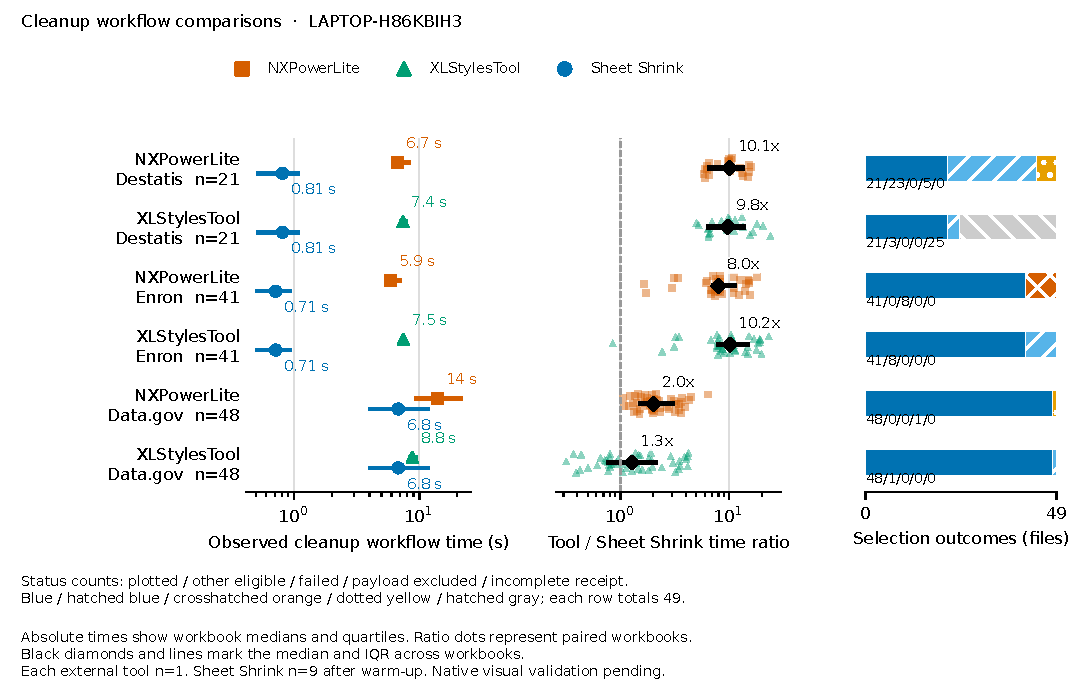
\includegraphics[width=\columnwidth]{figures/paired-cleanup-workflows.pdf}
\caption{Cleanup times and tool/SheetShrink ratios by corpus; parentheses give
pair counts. Time summaries and black ratio marks show medians and interquartile
ranges. NXPL: NXPowerLite; XLST: XLStylesTool; CP: Check Performance; INQ: Inquire.}
\label{fig:paired-cleanup-workflows}
\end{figure}


\subsection{Native validation of preservation rules}
\paragraph{Row-height preservation.}
In the Traffic workbook, promoting repeated empty-cell formatting into a row style
changed an automatically determined height from 12.75 to 9 points, shifting
subsequent content and changing 3,408 pixels in an independently specified reference
region. Requiring an explicit custom height before promotion restored byte-identical
native captures~\cite{rowpromotionfix}.

\paragraph{Font representatives.}
Two Destatis cases validate complementary font-preservation conditions. In a
higher-education workbook, removing 87 blank cells carrying explicit default-font and
no-fill metadata changed 25,640 pixels despite equal capture geometry and a
pixel-identical original-versus-original control. Retaining the required
representatives restored equality in an independently specified reference region.
Legacy print-name aliases were normalized for opening and recorded separately. In a
cultural-finance workbook, a blank cell's non-default font affected automatic row
height despite an omitted \texttt{applyFont} flag; a stored height without
\texttt{customHeight} did not prevent the change from 15 to 12.75 points. Retaining
the representative restored pixel and geometry equality in the independent control
and all 350 regions selected by the targeted capture policy.

\paragraph{Background definitions.}
In a Destatis horticulture workbook, SheetShrink reduced column definitions from
128,912 to 2,197. A corrected DeltaSieve background-envelope guard reduced the
capture selection from 16,101 to 165 regions; all 165 resulting image pairs were
pixel-identical.

\paragraph{Validation boundaries.}
In Wanderungen, excluding an empty trailing context row removed a spurious height
finding. All 37 captured image pairs were pixel-identical under the DeltaSieve
capture policy, while separate effective-height observations on two other worksheets
remained unresolved~\cite{trailingrowvalidation}.
These case studies validate specific preservation conditions within the recorded
capture scopes; they do not establish exhaustive workbook or corpus-wide visual
equivalence.

\subsection{Targeted visual outcomes on the Top49 selection}
A version-matched audit of the 49 workbooks with the largest absolute
SheetShrink reductions in each corpus retained 42 Destatis, 46 Data.gov,
and 46 Enron comparisons against the selected originals. Separately
documented normalized baselines supplied five further Destatis and two
further Enron observations. The remaining two, three, and one slots,
respectively, had no eligible observation. Across both baseline categories,
zero Destatis, seven Data.gov, and five Enron workbooks had recorded
differences. These counts describe the selected capture scope and include
findings whose cause remains unresolved. The five Enron workbooks had six
chart findings of 2--26 changed pixels with equal image dimensions and no
reported geometry change. The missing Enron workbook required repair
when opened in Excel, including after a separate legacy reconversion.

\subsection{Evidence boundary}
The selected controls demonstrate concrete preservation conditions and recorded
failures. They do not estimate corpus-wide defect prevalence. Reduction results
cover the frozen XLSX inventories. Matched cleanup-plus-opening measurements and
independent native references cover selected cases. Broader reference coverage
and matched whole-corpus cost remain open. Detailed development attempts, input hashes, native images and
producer versions remain in the source-linked artifact.

\section{Related Work}
\subsection{Workbook bloat and cleanup tools}
Microsoft Check Performance removes cells associated with unnecessary formatting
and other stored information from a loaded workbook~\cite{checkperformance}.
Its documentation warns that optimization can remove pixel-art cells. Inquire's
Clean Excess Cell Formatting command removes excess cells beyond the last
nonblank cell and can change conditional-formatting coverage~\cite{inquirecleanup}.
These documented policies motivate comparing both reduction and preservation
outcomes under explicit contracts.

Package-level cleanup also predates SheetShrink. XLStylesTool's developer
describes an Open-XML-based cleaner for excessive and corrupted styles that
operates independently of Excel's object model~\cite{xlstylestool}.
NXPowerLite Desktop 10 lists excess XLSX cell-format cleanup among its
features~\cite{nxpowerlite10}. Its engine description discusses formatted blank
cells as a source of large worksheet parts~\cite{nxengine}. These are relevant
comparison subjects. Their available descriptions do not establish the
guarded removal rules, compact row-font witnesses or native preservation
outcomes examined here. Those properties require version-specific evidence.
SheetShrink's positioning therefore includes its effect-aware rules, retained
representatives and measured costs alongside its execution before native loading.

\subsection{Spreadsheet loading and specialized parsing}
SheetReader studies specialized spreadsheet ingestion and the coupling of
parsing, decompression and parallel execution~\cite{sheetreader}. It motivates
evaluating loading cost and memory. SheetShrink produces an editable workbook
whose required layout and dependencies must survive package rewriting. Its
evaluation measures cleanup together with subsequent use of the output.

Mison combines structural indexing with speculative access to queried JSON
fields~\cite{mison}. Simdjson uses SIMD operations in a validating JSON
parser~\cite{simdjson}. These systems motivate efficient processing of
semi-structured representations. SheetShrink's document-rewriting obligation
additionally accounts for inheritance, references and native layout effects.

\subsection{Data transformation and spreadsheet refactoring}
Harris and Gulwani synthesize table transformations from example input/output
pairs~\cite{tableprog}. Potter's Wheel integrates interactive transformation and
discrepancy detection~\cite{potterswheel}. HoloClean repairs data through
probabilistic inference combining constraints and statistical evidence~\cite{holoclean}.
These systems infer or specify intended changes to data. SheetShrink's target
is removal of admitted package redundancy under a preservation contract.
Their data-repair accuracy measures therefore require a different ground truth
from our reduction, cost and preservation measurements.

Hermans et al. detect formula smells and suggest refactorings to improve
spreadsheet maintainability~\cite{formulasmells}. This is relevant to reasoning
about workbook structure and behavioral obligations. Formula readability and
refactoring objectives do not establish that empty cell records are removable
while retaining native layout. Execution outside Excel alone likewise leaves
the required effect analysis to be specified.

\subsection{Validation and dependency analysis}
Spreadsheet slicing integrates dependency reasoning with testing and
debugging~\cite{slicing}. Dependencies also constrain removal when retained
formulas or graphical objects refer to candidate content. Workbook comparison
tools provide observations about cell and format differences~\cite{spreadsheetcompare}.
Our native validation protocol uses DeltaSieve's region selection and capture
workflow~\cite{deltasievecompanion}, with independent references and mutation
controls to evaluate selected coverage. These validation mechanisms provide
evidence about cleanup outcomes after the package transformation.

\section{Discussion and Limitations}
The preservation contract is narrower than all possible spreadsheet behavior.
Rendering depends on the installed Excel version, fonts and calculation state.
A selected-region observation has limited scope. Unsupported XML and unsuccessful
opening or saving remain visible outcomes. The independent reference sample
estimates behavior on its eligible population and cannot establish a universal
absence of regressions.

Large reductions can coexist with small but important preservation structures.
A future Excel-hosted stage could replace font sentinels with measured custom
row heights and validate the replacement immediately. Such a stage has a native
application dependency and is outside the cleanup implementation examined here.
Whitespace removal likewise requires a separate justification of overflow and
layout effects. It is not assumed safe merely because a displayed value is blank.

The historical implementations explain the progression from diagnosis through
regular-expression cleanup to specialized byte-oriented execution. They are
useful engineering artifacts with distinct output behavior. Their age or slower
runtime does not establish that the current algorithm is correct.

Regression cases can support a reusable methodological observation when their
mechanism and control are retained. The Traffic example identifies a failure of
automatic-height style promotion, while the Migration example identifies an
exterior-context classification error in the validator. Their remedies operate
at different stages. Preserving that distinction prevents a validator change
from being reported as a cleaner improvement. Operational failures in the native
comparison environment also affect achieved evaluation coverage and belong in
the recorded outcomes even when cleanup itself completed quickly.

\section{Conclusion}
SheetShrink addresses spreadsheet redundancy through effect-aware removal and
compact preservation. Its implementation and evaluation distinguish compressed
size, XML changes, execution cost and observed presentation. The completed
manuscript must quantify those outcomes using the frozen experiments described
above and state the remaining unsupported cases.

\bibliographystyle{IEEEtran}
\bibliography{references}
\end{document}
